% Diagrama de Venn com três conjuntos
% Feito para o ÉguaTeX (eguatex.com.br). Uso livre (CC0 1.0).
%
% Compile e pronto: sai só a figura, em PDF.
% Para pôr no seu trabalho, use o PDF com \includegraphics ou copie
% o bloco tikzpicture para dentro de uma figure.
\documentclass[tikz,border=4pt]{standalone}
\usepackage[T1]{fontenc}
\usepackage{lmodern}
\usepackage{amsmath}

\colorlet{corA}{blue!30}
\colorlet{corB}{red!30}
\colorlet{corC}{green!35}
\colorlet{corRegiao}{black!45}

\begin{document}
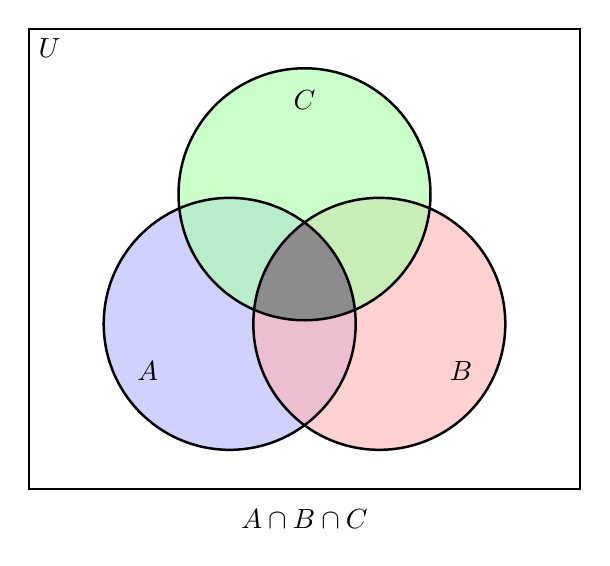
\begin{tikzpicture}[line cap=round]

% Mude estes números e textos.
\def\raio{1.6}   % raio de cada conjunto, em cm
\def\dist{1.9}   % distância entre os centros, em cm
\def\nomeA{$A$} \def\nomeB{$B$} \def\nomeC{$C$} \def\nomeU{$U$}
\def\legenda{$A\cap B\cap C$}

\def\conjA{(90+120:{\dist/1.732}) circle[radius=\raio]}
\def\conjB{(90-120:{\dist/1.732}) circle[radius=\raio]}
\def\conjC{(90:{\dist/1.732}) circle[radius=\raio]}

% cores dos conjuntos, transparentes para mostrar as sobreposições
\fill[corA, opacity=0.6] \conjA;
\fill[corB, opacity=0.6] \conjB;
\fill[corC, opacity=0.6] \conjC;

% Região destacada: interseção dos três. Apague o bloco para tirar.
\begin{scope}\clip \conjA; \clip \conjB; \fill[corRegiao] \conjC; \end{scope}

% contornos e nomes
\draw[line width=0.9pt] ({-\dist-\raio},{-\dist/1.732/2-\raio-0.5}) rectangle ({\dist+\raio},{\dist/1.732+\raio+0.5});
\node[anchor=north west] at ({-\dist-\raio},{\dist/1.732+\raio+0.5}) {\nomeU};
\draw[line width=0.9pt] \conjA;
\draw[line width=0.9pt] \conjB;
\draw[line width=0.9pt] \conjC;
\node at (210:{\dist/1.732+0.75*\raio}) {\nomeA};
\node at (-30:{\dist/1.732+0.75*\raio}) {\nomeB};
\node at (90:{\dist/1.732+0.75*\raio}) {\nomeC};
\node[below=4pt] at (0,{-\dist/1.732/2-\raio-0.5}) {\legenda};
\end{tikzpicture}
\end{document}
